\section{Рабочий проект}

\subsection{Спецификация компонентов и классов программы}

\subsubsection{Модуль main.py}

Модуль предоставляет графический интерфейс с меню для переключения между тремя режимами работы: анализ изображений, обучение и тестирование нейронной сети. 

Класс -- MainWindow.

Описание класса MainWindow.
Класс предназначен для управления главным окном приложения и переключения между режимами работы программы. Базовый класс -- QMainWindow, стандартный класс библиотеки PyQt5. Интерфейсы: панель меню, позволяющая переключать режимы работы программы; центральный виджет QStackedWidget, отображающий интерфейс активного режима работы. Константы: отсутствуют. Внутренние поля представлены в таблице~\ref{table:main_widgets}.

\begin{xltabular}{\textwidth}{|X|X|X|}
	\caption{Внутренние поля класса MainWindow\label{table:main_widgets}} \\
	\hline 
	\centrow Внутреннее поле & 
	\centrow Тип & 
	\centrow Описание \\ 
	\hline 
	\endfirsthead
	
	\caption*{Продолжение таблицы \ref{table:main_widgets}} \\
	\hline 
	\centrow Внутреннее поле & 
	\centrow Тип & 
	\centrow Описание \\ 
	\hline 
	\endhead
	
	stack & QStackedWidget & Содержит три виджета графического интерфейса для каждого режима работы программы \\ \hline
	analysis\_widget & ImageAnalysisWidget & Виджет, содержащий графический интерфейс режима анализа изображений \\ \hline
	training\_widget & TrainingWidget & Виджет, содержащий графический интерфейс режима обучения нейронной сети \\ \hline
	testing\_widget & TestingWidget & Виджет, содержащий графический интерфейс режима тестирования нейронной сети \\ \hline
\end{xltabular}
Методы класса представлены в таблице~\ref{table:main_method}.
\renewcommand{\arraystretch}{0.8} % уменьшение расстояний до сетки таблицы
\begin{xltabular}{\textwidth}{|>{\hsize=0.7\hsize\raggedright\arraybackslash}X|
		>{\hsize=1.0\hsize\setlength{\baselineskip}{0.7\baselineskip}}X|
		>{\hsize=1.0\hsize}X|
		>{\hsize=1.3\hsize}X|}
	\caption{Методы класса MainWindow\label{table:main_method}}\\
	\hline 
	\centrow \setlength{\baselineskip}{0.7\baselineskip} Название метода & 
	\centrow Параметры метода &
	\centrow Возвращаемое значение & 
	\centrow Назначение метода \\ 
	\hline 
	\endfirsthead
	
	\caption*{Продолжение таблицы \ref{table:main_method}}\\
	\hline 
	\centrow Название метода & 
	\centrow Параметры метода &
	\centrow Возвращаемое значение & 
	\centrow Назначение метода \\ 
	\hline 
	\endhead
	
	\_\_init\_\_ & Не имеет & Не имеет  & Инициализирует главное окно программы, задает его параметры, заголовок, панель меню с действиями для переключения режимов \\ \hline 
	switch\_mode & index --  идентификатор  активного режима окна& Не имеет& Переключает графический интерфейс в соответствии с выбранным режимом работы \\ \hline
	
\end{xltabular}
\renewcommand{\arraystretch}{1.0} % восстановление сетки
\vspace{-\baselineskip}

\subsubsection{Модуль model.py}

Модуль определяет структуру нейронной сети UNet, используемой для обнаружения разливов нефти.

Класс -- UNet.

Описание класса UNet.
Класс реализует модель UNet для сегментации и распознавания пятен нефтяных разливов на поверхности водоемов. Базовый класс --  nn.Module, стандартный класс библиотеки PyTorch. Интерфейсы: общедоступные методы \_\_init\_\_ и forward. Константы отсутствуют. Внутренние поля представлены в таблице~\ref{table:network_components}.
\begin{xltabular}{\textwidth}{|X|X|X|}
	\caption{Внутренние поля класса UNet \label{table:network_components}} \\
	\hline 
	\centrow Внутреннее поле & 
	\centrow Тип & 
	\centrow Описание \\ 
	\hline 
	\endfirsthead
	
	\caption*{Продолжение таблицы \ref{table:network_components}} \\
	\hline 
	\centrow Внутреннее поле & 
	\centrow Тип & 
	\centrow Описание \\ 
	\hline 
	\endhead
	
	enc1 & nn.Sequential & Первый блок энкодера \\ \hline
	enc2 & nn.Sequential & Второй блок энкодера \\ \hline
	pool & nn.MaxPool2d & Слой максимального пуллинга, уменьшающий разрешение \\ \hline
	bottleneck & nn.Sequential & Блок узкого места \\ \hline
	upconv2 & nn.ConvTranspose2d & Второй слой повышения разрешения \\ \hline
	dec2 & nn.Sequential & Второй блок декодера \\ \hline
	upconv1 & nn.ConvTranspose2d & Первый слой повышения разрешения \\ \hline
	dec1 & nn.Sequential & Первый блок декодера \\ \hline
	final\_conv & nn.Conv2d & Финальный сверточный слой, создающий выходную маску признаков \\ \hline
\end{xltabular}
Методы класса представлены в таблице~\ref{table:model_method}.
\renewcommand{\arraystretch}{0.8} % уменьшение расстояний до сетки таблицы
\begin{xltabular}{\textwidth}{|>{\hsize=0.7\hsize\raggedright\arraybackslash}X|
		>{\hsize=1.0\hsize\setlength{\baselineskip}{0.7\baselineskip}}X|
		>{\hsize=1.0\hsize}X|
		>{\hsize=1.3\hsize}X|}
	\caption{Методы класса UNet\label{table:model_method}}\\
	\hline 
	\centrow Название метода & 
	\centrow Параметры метода & 
	\centrow Возвращаемое значение &
	\centrow Назначение метода \\ 
	\hline 
	\endfirsthead
	
	\caption*{Продолжение таблицы \ref{table:model_method}}\\
	\hline 
	\centrow Название метода & 
	\centrow Параметры метода & 
	\centrow Возвращаемое значение &
	\centrow Назначение метода \\ 
	\hline 
	\endhead
	
	\_\_init\_\_ & \parbox[t]{\linewidth}{in\_channels -- количество входных каналов; \\ out\_channels -- количество выходных каналов}  & Не имеет & Инициализирует архитектуру UNet \\ \hline 
	forward & x -- входной тензор & torch.Tensor -- выходная маска признаков & Выполняет прямой проход через нейронную сеть, возвращая итог сегментации \\ \hline
	conv\_block & \parbox[t]{\linewidth}{ in\_c --  входные каналы; \\ out\_c -- выходные каналы}& nn.Sequential -- контейнер сверточного блока & Определяет сверточный блок с двумя сверточными слоями и функциями активации\\ \hline
	
\end{xltabular}
\renewcommand{\arraystretch}{1.0} % восстановление сетки
\vspace{-\baselineskip}

\subsubsection{Модуль test.py}

Модуль содержит функции для оценки обученной модели UNet на одном изображении.  Не содержит классов. Методы модуля:
\begin{enumerate}
	\item dice\_coefficient. Вычисляет коэффициент Dice для предсказанной маски. Входные данные:
	\begin{itemize}
		\item pred (тип torch.Tensor) -- предсказанная маска;
		\item target (тип torch.Tensor ) -- целевая маска;
		\item smooth (тип float,  значение по умолчанию -- 1e$^{-6} $) -- стабилизирующая константа для избежания деления на ноль.
	\end{itemize}
	Возвращаемые данные -- коэффициент Dice в виде float-числа.
	\item iou\_score. Вычисляет пересечение по объединению (коэффициент IoU) для предсказанной маски. Входные данные:
	\begin{itemize}
		\item pred (тип torch.Tensor) -- предсказанная маска;
		\item target (тип torch.Tensor ) -- целевая маска;
		\item smooth (тип float,  значение по умолчанию -- 1e$^{-6} $) -- стабилизирующая константа для избежания деления на ноль.
	\end{itemize}
	Возвращаемые данные -- коэффициент пересечения по объединению в виде float-числа.
	\item load\_image. Загружает изображение и выполняет предобработку для дальнейшего анализа нейронной сетью. Входные данные:
	\begin{itemize}
		\item path (тип str) -- путь к загружаемому изображению;
		\item size (тип tuple) -- целевой размер изображения для дальнейшей обработки нейронной сетью.
	\end{itemize}
	Возвращаемые данные: нормализованный массив изображения типа np.ndarray.
	\item run\_evaluation. Выполняет оценку точности обученной модели нейронной сети и возвращает результаты обработки и метрики. Входные данные:
	\begin{itemize}
		\item image\_path (тип str) -- путь к анализируемому изображению;
		\item weights (тип str) -- путь к оцениваемым весам модели;
		\item threshold (тип float, значение по умолчанию = 0,5) -- порог для бинаризации масок
	\end{itemize}
	Возвращаемые данные -- значения коэффициентов Dice и IoU, исходное изображение, ожидаемую маску, полученную при помощи пороговой бинаризации и предсказанную сетью маску в виде словаря dict.
\end{enumerate}

\subsubsection{Модуль train.py}

Модуль управляет загрузкой датасета и обучением нейронной сети.

Классы: dataset и Trainer.

Описание класса dataset.
Класс загружает и предобрабатывает изображения и создает псевдомаски на основании порога для обучения нейронной сети. Базовый класс -- Dataset, стандартный класс библиотеки PyTorch. Интерфейсы -- общедоступные методы \_\_init\_\_, \_\_len\_\_, \_\_getitem\_\_, общедоступные атрибуты image\_dir, images. Константы отсутствуют. Внутренние поля представлены в таблице~\ref{table:dataset_params}.
\begin{xltabular}{\textwidth}{|X|X|X|}
	\caption{Внутренние поля класса dataset \label{table:dataset_params}} \\
	\hline 
	\centrow Внутреннее поле & 
	\centrow Тип & 
	\centrow Описание \\ 
	\hline 
	\endfirsthead
	
	\caption*{Продолжение таблицы \ref{table:dataset_params}} \\
	\hline 
	\centrow Внутреннее поле & 
	\centrow Тип & 
	\centrow Описание \\ 
	\hline 
	\endhead
	
	image\_dir & str & Папка, содержащая датасет \\ \hline
	images & list & Список имен файлов изображений для обучения \\ \hline
	threshold & float & Порог для создания обучающих масок \\ \hline
\end{xltabular}
Методы класса представлены в таблице~\ref{table:dataset_method}. 
\renewcommand{\arraystretch}{0.8} % уменьшение расстояний до сетки таблицы
\begin{xltabular}{\textwidth}{|>{\hsize=0.7\hsize\raggedright\arraybackslash}X|
		>{\hsize=1.0\hsize\setlength{\baselineskip}{0.7\baselineskip}}X|
		>{\hsize=1.0\hsize}X|
		>{\hsize=1.3\hsize}X|}
	\caption{Методы класса dataset\label{table:dataset_method}}\\
	\hline 
	\centrow Название метода & 
	\centrow Параметры метода & 
	\centrow Возвращаемое значение &
	\centrow Назначение метода \\ 
	\hline 
	\endfirsthead
	
	\caption*{Продолжение таблицы \ref{table:dataset_method}}\\
	\hline 
	\centrow Название метода & 
	\centrow Параметры метода & 
	\centrow Возвращаемое значение &
	\centrow Назначение метода \\ 
	\hline 
	\endhead
	
	\_\_init\_\_ & \parbox[t]{\linewidth}{image\_dir -- путь к папке с датасетом; \\ threshold -- порог для создания обучающих масок} & Не имеет & Инициализирует датасет, проверяя директорию и загружая имена файлов изображений \\ \hline 
	\_\_len\_\_ & Не имеет & Количество изображений в датасете & Определяет количество изображений в датасете \\ \hline
	\_\_getitem\_\_ & idx -- порядковый номер обрабатываемого изображения & тензор изображения и маски & Загружает, предобрабатывает и создает обучающую маску для изображений датасета \\ \hline
	
\end{xltabular}
\renewcommand{\arraystretch}{1.0} % восстановление сетки
\vspace{-\baselineskip}

Описание класса Trainer.
Класс управляет обучением модели нейронной сети и отправляет сигналы о состоянии процесса обучения для обновления графического интерфейса. Базовый класс -- QObject, стандартный класс библиотеки PyQt5. Интерфейсы -- сигналы о состоянии процесса обучения, общедоступный метод \_\_init\_\_. Константы отсутствуют. Внутренние поля представлены в таблице~\ref{table:training_signals}.
\begin{xltabular}{\textwidth}{|X|X|X|}
	\caption{Внутренние поля класса Trainer\label{table:training_signals}}\\
	\hline 
	\centrow Внутреннее поле & 
	\centrow Тип & 
	\centrow Описание \\ 
	\hline 
	\endfirsthead
	
	\caption*{Продолжение таблицы \ref{table:training_signals}}\\
	\hline 
	\centrow Внутреннее поле & 
	\centrow Тип & 
	\centrow Описание \\ 
	\hline 
	\endhead
	
	\hline 
	\endfoot
	
	epoch\_start\_signal & pyqtSignal[int, int] & сигнал начала эпохи, содержащий её номер и общее количество эпох \\ \hline
	epoch\_complete\_signal & pyqtSignal[int, float] & сигнал завершения эпохи, содержащий её номер и среднее значение потери при обучении \\ \hline
	batch\_progress\_signal & pyqtSignal[int, int, float] & сигнал прогресса обработки батча, содержащий его номер, потерю, общее число батчей \\ \hline
	training\_complete\_signal & pyqtSignal[str] & сигнал завершения обучения \\ \hline
\end{xltabular}
Методы класса представлены в таблице~\ref{table:Trainer_method}.
\renewcommand{\arraystretch}{0.8} % уменьшение расстояний до сетки таблицы
\begin{xltabular}{\textwidth}{|>{\hsize=0.7\hsize\raggedright\arraybackslash}X|
		>{\hsize=1.0\hsize\setlength{\baselineskip}{0.7\baselineskip}}X|
		>{\hsize=1.0\hsize}X|
		>{\hsize=1.3\hsize}X|}
	\caption{Методы класса Trainer\label{table:Trainer_method}}\\
	\hline 
	\centrow \setlength{\baselineskip}{0.7\baselineskip} Название метода & 
	\centrow Параметры метода & 
	\centrow Возвращаемое значение & 
	\centrow Назначение метода \\ 
	\hline 
	\endfirsthead
	
	\caption*{Продолжение таблицы \ref{table:Trainer_method}}\\
	\hline 
	\centrow Название метода & 
	\centrow Параметры метода & 
	\centrow Возвращаемое значение &
	\centrow Назначение метода \\ 
	\hline 
	\endhead
	
	\_\_init\_\_ & \parbox[t]{\linewidth}{image\_dir -- путь датасета; \\ save\_path -- путь сохранения весов; \\ batch\_size -- размер батча; \\ epochs -- количество эпох;\\  lr -- скорость обучения; \\ threshold -- порог для обучающих масок}  & Не имеет & Инициализирует процесс обучения с определенными параметрами \\ \hline 
	run & Не имеет & Не имеет & Обучает нейронную сеть, отправляя сигналы о прогрессе, и сохраняет параметры модели по завершении обучения \\ \hline
	
\end{xltabular}
\renewcommand{\arraystretch}{1.0} % восстановление сетки
\vspace{-\baselineskip}

В модуле train.py также реализован метод main(), предназначенная для получения аргументов обучения из графического интерфейса и запуска обучения при помощи Trainer. Метод не имеет входных и возвращаемых данных.

\subsubsection{Модуль detect.py}

Модуль используется для анализа изображений с использованием обученной модели нейронной сети, обнаруживая и выделяя пятна нефтяных разливов.  Не содержит классов. Методы модуля:
\begin{enumerate}
	\item load\_model. Загружает и инициализирует модель нейронной сети с указанными параметрами. Входные данные -- model\_path (тип str) -- путь к файлу параметров модели. Возвращаемые данные -- элемент класса Unet модуля model.py с загруженными из файла весами.
	\item analyze\_return. Метод обрабатывает изображение, используя нейронную сеть, создает бинарную маску разлива и возвращает исходное изображение с выделенными распознанными пятнами нефтяных разливов. Входные данные:
	\begin{itemize}
		\item image\_path (тип str) -- путь к анализируемому изображению;
		\item model\_path (тип str) -- путь к файлу параметров нейронной сети;
		\item threshold (тип float, значение по умолчанию -- 0,5) -- порог для бинаризации маски.
	\end{itemize}
	Возвращаемые данные -- изображение с выделенными распознанными нефтяными пятнами в формате np.ndarray.
\end{enumerate}

\subsubsection{Модуль analyze\_ui.py}

Модуль содержит графический интерфейс режима анализа изображений с использованием предварительно обученной модели нейронной сети.

Класс -- ImageAnalysisWidget. 

Описание класса ImageAnalysisWidget.
Класс содержит графический интерфейс, позволяющий выбрать анализируемое изображение, файл параметров нейронной сети, запустить процесс анализа и сохранить результат и отображающий этот результат. Базовый класс -- QWidget, стандартный класс библиотеки PyQt5. Интерфейсы -- поля для путей к изображению и модели, кнопки для выбора этих путей, начала анализа, сохранения результата, область отображения изображения. Константы отсутствуют. Внутренние поля класса представлены в таблице~\ref{table:image_analysis_elements}.
\begin{xltabular}{\textwidth}{|X|X|X|}
	\caption{Внутренние поля класса ImageAnalysisWidget\label{table:image_analysis_elements}}\\
	\hline 
	\centrow Внутреннее поле & 
	\centrow Тип & 
	\centrow Описание \\ 
	\hline 
	\endfirsthead
	
	\caption*{Продолжение таблицы \ref{table:image_analysis_elements}}\\
	\hline 
	\centrow Внутреннее поле & 
	\centrow Тип & 
	\centrow Описание \\ 
	\hline 
	\endhead
	
	\hline 
	\endfoot
	
	image\_path & str & путь к выбранному изображению \\ \hline
	model\_path & str & путь к выбранному файлу параметров нейронной сети \\ \hline
	result\_img & np.ndarray & проанализированное изображение с разметкой \\ \hline
	path\_label & QLabel & надпись "Изображение для анализа:" \\ \hline
	path\_field & QTextEdit & текстовое поле для отображения пути к изображению \\ \hline
	select\_button & QPushButton & кнопка для выбора изображения \\ \hline
	model\_label & QLabel & надпись "Путь к модели нейросети:" \\ \hline
	model\_path\_field & QTextEdit & текстовое поле для отображения пути к модели \\ \hline
	select\_model\_button & QPushButton & кнопка для выбора файла параметров \\ \hline
	image\_label & QLabel & поле для отображения изображения \\ \hline
	analyze\_button & QPushButton & кнопка для анализа изображения \\ \hline
	save\_button & QPushButton & кнопка для сохранения результата анализа \\ \hline
\end{xltabular}
Методы класса представлены в таблице~\ref{table:analyze_ui_method}.
\renewcommand{\arraystretch}{0.8} % уменьшение расстояний до сетки таблицы
\begin{xltabular}{\textwidth}{|>{\hsize=0.7\hsize\raggedright\arraybackslash}X|
		>{\hsize=1.0\hsize\setlength{\baselineskip}{0.7\baselineskip}}X|
		>{\hsize=1.0\hsize}X|
		>{\hsize=1.3\hsize}X|}
	\caption{Методы класса ImageAnalysisWidget\label{table:analyze_ui_method}}\\
	\hline 
	\centrow \setlength{\baselineskip}{0.7\baselineskip} Название метода & 
	\centrow Параметры метода & 
	\centrow Возвращаемое значение & 
	\centrow Назначение метода \\ 
	\hline 
	\endfirsthead
	
	\caption*{Продолжение таблицы \ref{table:analyze_ui_method}}\\
	\hline 
	\centrow Название метода & 
	\centrow Параметры метода & 
	\centrow Возвращаемое значение &
	\centrow Назначение метода \\ 
	\hline 
	\endhead
	
	\_\_init\_\_ & Не имеет & Не имеет  & Инициализирует графический интерфейс, включая его макет и элементы  \\ \hline 
	select\_image & Не имеет & Не имеет & Открывает диалоговое окно выбора изображения, отображает путь к нему и само изображение в интерфейсе \\ \hline
	select\_model & Не имеет & Не имеет & Открывает диалоговое окно выбора файла настроек модели и отображает путь к нему \\ \hline
	\parbox[t]{\linewidth}{analyze\_ \\ image} & Не имеет & Не имеет & Анализирует загруженное изображение при помощи нейронной сети и отображает результат распознавания \\ \hline
	save\_result & Не имеет & Не имеет & Открывает диалоговое окно выбора папки сохранения результата анализа изображения и сохраняет результат \\ \hline
	
\end{xltabular}
\renewcommand{\arraystretch}{1.0} % восстановление сетки
\vspace{-\baselineskip}

\subsubsection{Модуль train\_ui.py}

Модуль содержит графический интерфейс для настройки параметров и запуска процесса обучения модели нейронной сети.

Классы: TrainingThread, TrainingWidget.

Описание класса TrainingThread.
Данный класс выполняет процесс обучений нейронной сети в отдельном потоке для избежания блокировки и зависания графического интерфейса. Базовый класс -- QThread, стандартный класс библиотеки PyQt5. Интерфейсы -- сигналы для передачи прогресса обучения и обработки ошибок, функция, управляющая процессом обучения. Константы отсутствуют. Внутренние поля представлены в таблице~\ref{table:training_components}.
\begin{xltabular}{\textwidth}{|X|X|X|}
	\caption{Внутренние поля класса TrainingThread\label{table:training_components}}\\
	\hline 
	\centrow Внутреннее поле & 
	\centrow Тип & 
	\centrow Описание \\ 
	\hline 
	\endfirsthead
	
	\caption*{Продолжение таблицы \ref{table:training_components}}\\
	\hline 
	\centrow Внутреннее поле & 
	\centrow Тип & 
	\centrow Описание \\ 
	\hline 
	\endhead
	
	\hline 
	\endfoot
	
	trainer & Trainer & экземпляр класса Trainer из train.py для обучения нейронной сети \\ \hline
	error\_signal & pyqtSignal[str] & сигнал для передачи сообщений об ошибках в процессе обучения \\ \hline
\end{xltabular}
Методы класса представлены в таблице~\ref{table:TrainingThread_method}.
\renewcommand{\arraystretch}{0.8} % уменьшение расстояний до сетки таблицы
\begin{xltabular}{\textwidth}{|>{\hsize=0.7\hsize\raggedright\arraybackslash}X|
		>{\hsize=1.0\hsize\setlength{\baselineskip}{0.7\baselineskip}}X|
		>{\hsize=1.0\hsize}X|
		>{\hsize=1.3\hsize}X|}
	\caption{Методы класса TrainigThread\label{table:TrainingThread_method}}\\
	\hline 
	\centrow \setlength{\baselineskip}{0.7\baselineskip} Название метода & 
	\centrow Параметры метода & 
	\centrow Возвращаемое значение & 
	\centrow Назначение метода \\ 
	\hline 
	\endfirsthead
	
	\caption*{Продолжение таблицы \ref{table:TrainingThread_method}}\\
	\hline 
	\centrow Название метода & 
	\centrow Параметры метода & 
	\centrow Возвращаемое значение &
	\centrow Назначение метода \\ 
	\hline 
	\endhead
	
	\_\_init\_\_ & \parbox[t]{\linewidth}{dataset\_path -- путь к датасету; \\ model\_path -- путь к директории сохранения модели; \\ batch\_size -- размер батча; \\ epochs -- количество эпох обучения}  & Не имеет & Инициализирует поток обучения нейронной сети с экземпляром класса Trainer  \\ \hline 
	run & Не имеет & Не имеет & Выполняет обучение нейронной сети с обработкой ошибок \\ \hline
	
\end{xltabular}
\renewcommand{\arraystretch}{1.0} % восстановление сетки
\vspace{-\baselineskip}

Описание класса TrainingWidget.
Класс предоставляет графиеский интерфейс для выбора параметров обучения и отображения прогресса. Базовый класс -- QWidget, стандартный класс PyQt5. Интерфейсы -- поля ввода расположений датасета и сохранения результата, кнопки выбора путей, запуска обучения, шкала прогресса завершения обучения, текстовое поле для отображения сведений об обучении. Константы отсутствуют. Внутренние поля представлены в таблице~\ref{table:training_interface}.
\begin{xltabular}{\textwidth}{|X|X|X|}
	\caption{Внутренние поля класса TrainingWidget\label{table:training_interface}}\\
	\hline 
	\centrow Внутреннее поле & 
	\centrow Тип & 
	\centrow Описание \\ 
	\hline 
	\endfirsthead
	
	\caption*{Продолжение таблицы \ref{table:training_interface}}\\
	\hline 
	\centrow Внутреннее поле & 
	\centrow Тип & 
	\centrow Описание \\ 
	\hline 
	\endhead
	
	\hline 
	\endfoot
	
	dataset\_label & QLabel & надпись "<Папка датасета:>"\\ \hline
	dataset\_path\_field & QTextEdit & поле для отображения выбранной папки датасета \\ \hline
	select\_dataset\_button & QPushButton & кнопка для выбора папки датасета \\ \hline
	model\_label & QLabel & надпись "<Папка сохранения:>" \\ \hline
	model\_path\_field & QTextEdit & поле для отображения выбранной папки сохранения \\ \hline
	select\_model\_button & QPushButton & кнопка для выбора папки сохранения \\ \hline
	batch\_size\_label & QLabel & надпись "<Размер батча:>" \\ \hline
	batch\_size\_combo & QComboBox & выпадающий список для выбора размера батча \\ \hline
	epochs\_label & QLabel & надпись "Количество эпох:" \\ \hline
	epochs\_field & QLineEdit & поле для ввода количества эпох обучения \\ \hline
	progress\_label & QLabel & надпись "Прогресс эпохи:" \\ \hline
	progress\_bar & QProgressBar & шкала прогресса обучения нейронной сети \\ \hline
	log\_label & QLabel & надпись "Процесс выполнения:" \\ \hline
	output\_text & QTextEdit & поле для отображения сведений о процессе обучения \\ \hline
	train\_button & QPushButton & кнопка для запуска обучения \\ \hline
	thread & TrainingThread & поток для процесса обучения \\ \hline
\end{xltabular}
Методы класса представлены в таблице~\ref{table:TrainingWidget_method}.
\renewcommand{\arraystretch}{0.8} % уменьшение расстояний до сетки таблицы
\begin{xltabular}{\textwidth}{|>{\hsize=0.7\hsize\raggedright\arraybackslash}X|
		>{\hsize=1.0\hsize\setlength{\baselineskip}{0.7\baselineskip}}X|
		>{\hsize=1.0\hsize}X|
		>{\hsize=1.3\hsize}X|}
	\caption{Методы класса TrainigWidget\label{table:TrainingWidget_method}}\\
	\hline 
	\centrow \setlength{\baselineskip}{0.7\baselineskip} Название метода & 
	\centrow Параметры метода & 
	\centrow Возвращаемое значение &  
	\centrow Назначение метода \\ 
	\hline 
	\endfirsthead
	
	\caption*{Продолжение таблицы \ref{table:TrainingWidget_method}}\\
	\hline 
	\centrow Название метода & 
	\centrow Параметры метода & 
	\centrow Возвращаемое значение & 
	\centrow Назначение метода \\ 
	\hline 
	\endhead
	
	\_\_init\_\_ & Не имеет & Не имеет  & Инициализирует графический интерфейс, включая макет и элементы для настройки обучения и отображения прогресса  \\ \hline 
	\parbox[t]{\linewidth}{select\_dataset \\ \_folder} & Не имеет & Не имеет & Открывает диалоговое окно для выбора папки, содержащей датасет \\ \hline
	\parbox[t]{\linewidth}{select\_model\\ \_path} & Не имеет & Не имеет & Открывает диалоговое окно для выбора папки сохранения весов обученной нейронной сети \\ \hline
	run\_training & Не имеет & Не имеет & Проверяет корректность параметров обучения, заданных пользователем, отображает ошибки при наличии, создает поток обучения, подключает сигналы для обновления графического интерфейса \\ \hline
	\parbox[t]{\linewidth}{on\_epoch\_ \\ start} & \parbox[t]{\linewidth}{epoch -- номер текущей эпохи обучения; \\ total\_epochs -- общее количество эпох} & Не имеет & Обновляет отображаемый журнал обучения нейронной сети записью о начале эпохи и сбрасывает шкалу прогресса при начале новой эпохи обучения \\ \hline
	\parbox[t]{\linewidth}{on\_epoch\_ \\ complete} & \parbox[t]{\linewidth}{epoch -- номер завершенной эпохи; \\ avg\_loss -- среднее значение потери за эпоху обучения} & Не имеет & Обновляет отображаемый журнал информацией о завершении эпохи и заполняет шкалу прогресса по окончании эпохи обучения\\ \hline
	\parbox[t]{\linewidth}{on\_batch\_ \\ progress} & \parbox[t]{\linewidth}{batch -- номер текущего батча; \\ total\_batches -- общее количество батчей; \\ loss -- значение потери для текущего батча} & Не имеет & Обновляет шкалу прогресса в процессе обучения \\ \hline
	\parbox[t]{\linewidth}{append\_ \\ output} & text --  текст, добавляемый в журнал обучения& Не имеет & Добавляет текст в область отображения журнала \\ \hline
	show\_error & error\_message --  отображаемое сообщение об ошибке & Не имеет & Отображает диалоговое окно ошибки \\ \hline
	
\end{xltabular}
\renewcommand{\arraystretch}{1.0} % восстановление сетки
\vspace{-\baselineskip}

\subsubsection{Модуль test\_ui.py}

Модуль предоставляет графический интерфейс для тестирования модели нейронной сети.

Классы: TestingThread, TestingWidget.

Описание класса TestingThread.
Класс выполняет оценку модели в отдельном потоке, чтобы избежать зависаний графического интерфейса. Базовый класс -- QThread, стандартный класс PyQt5. Интерфейсы класса -- сигналы для обновления графического интерфейса. Константы отсутствуют. Внутренние поля представлены в таблице~\ref{table:testing_components}.
\begin{xltabular}{\textwidth}{|X|X|X|}
	\caption{Внутренние поля класса TestingThread\label{table:testing_components}}\\
	\hline 
	\centrow Внутреннее поле & 
	\centrow Тип & 
	\centrow Описание \\ 
	\hline 
	\endfirsthead
	
	\caption*{Продолжение таблицы \ref{table:testing_components}}\\
	\hline 
	\centrow Внутреннее поле & 
	\centrow Тип & 
	\centrow Описание \\ 
	\hline 
	\endhead
	
	\hline 
	\endfoot
	
	image\_path & str & путь к тестовому изображению \\ \hline
	model\_path & str & путь к файлу настроек модели нейронной сети \\ \hline
	output\_signal & pyqtSignal[str] & сигнал для сообщений о результатах тестирования \\ \hline
	results\_signal & pyqtSignal[dict] & сигнал для передачи результатов оценки \\ \hline
	error\_signal & pyqtSignal[str] & сигнал для сообщений об ошибках тестирования \\ \hline
\end{xltabular}
Методы класса представлены в таблице~\ref{table:TestingThread_method}.
\renewcommand{\arraystretch}{0.8} % уменьшение расстояний до сетки таблицы
\begin{xltabular}{\textwidth}{|>{\hsize=0.7\hsize\raggedright\arraybackslash}X|
		>{\hsize=1.0\hsize\setlength{\baselineskip}{0.7\baselineskip}}X|
		>{\hsize=1.0\hsize}X|
		>{\hsize=1.3\hsize}X|}
	\caption{Методы класса TestingThread\label{table:TestingThread_method}}\\
	\hline 
	\centrow \setlength{\baselineskip}{0.7\baselineskip} Название метода & 
	\centrow Параметры метода & 
	\centrow Возвращаемое значение &  
	\centrow Назначение метода \\ 
	\hline 
	\endfirsthead
	
	\caption*{Продолжение таблицы \ref{table:TestingThread_method}}\\
	\hline 
	\centrow Название метода & 
	\centrow Параметры метода & 
	\centrow Возвращаемое значение & 
	\centrow Назначение метода \\ 
	\hline 
	\endhead
	
	\_\_init\_\_ &  \parbox[t]{\linewidth}{image\_path -- путь к тестовому изображению; \\ model\_path -- путь к файлу параметров нейронной сети} & Не имеет  & Инициализирует поток, передавая в него пути к тестовому изображению и папке модели  \\ \hline 
	run & Не имеет & Не имеет & Выполняет оценку нейронной сети, отправляя результаты или ошибки через сигналы  \\ \hline
	
\end{xltabular}
\renewcommand{\arraystretch}{1.0} % восстановление сетки
\vspace{-\baselineskip}

Описание класса TestingWidget.
Класс содержит графический интерфейс для выбора тестового изображения и файла весов модели, запуска оценки и отображения полученных метрик точности нейронной сети, целевой и предсказанной масок. Базовый класс -- QWidget, стандартный класс PyQt5. Интерфейсы класса -- поля для отображения путей к тестовому изображению и файлу весов, кнопки для выбора этих файлов и запуска тестирования, области для отображения изображений и метрик. Константы отсутствуют. Внутренние поля представлены в таблице~\ref{table:testing_interface}.
\begin{xltabular}{\textwidth}{|X|X|X|}
	\caption{Внутренние поля класса TestingWidget\label{table:testing_interface}}\\
	\hline 
	\centrow Внутреннее поле & 
	\centrow Тип & 
	\centrow Описание \\ 
	\hline 
	\endfirsthead
	
	\caption*{Продолжение таблицы \ref{table:testing_interface}}\\
	\hline 
	\centrow Внутреннее поле & 
	\centrow Тип & 
	\centrow Описание \\ 
	\hline 
	\endhead
	
	\hline 
	\endfoot
	
	image\_path & str & путь к тестовому изображению \\ \hline 
	model\_path & str & путь к тестируемым параметрам модели \\ \hline 
	path\_label & QLabel & надпись "Изображение для проверки модели:" \\ \hline 
	image\_path\_field & QTextEdit & поле для отображения пути к изображению \\ \hline 
	select\_image\_button & QPushButton & кнопка выбора изображения \\ \hline 
	model\_label & QLabel & надпись "Путь к параметрам нейросети:" \\ \hline 
	model\_path\_field & QTextEdit & поле для отображения пути к параметрам модели \\ \hline 
	select\_model\_button & QPushButton & кнопка выбора модели \\ \hline 
	output\_text & QTextEdit & поле для вывода метрик точности \\ \hline 
	input\_text\_label & QLabel & надпись "Исходное изображение" \\ \hline 
	input\_image\_label & QLabel & поле отображения входного изображения \\ \hline 
	gt\_text\_label & QLabel & надпись "Ожидаемый результат" \\ \hline 
	gt\_mask\_label & QLabel & поле отображения эталонной маски \\ \hline 
	pred\_text\_label & QLabel & надпись "Результат работы модели" \\ \hline 
	pred\_mask\_label & QLabel & поле отображения предсказанной маски \\ \hline 
	test\_button & QPushButton & кнопка запуска тестирования \\ \hline 
	thread & TestingThread & поток выполнения тестирования \\ \hline
\end{xltabular}
Методы класса представлены в таблице~\ref{table:TestingWidget_method}.
\renewcommand{\arraystretch}{0.8} % уменьшение расстояний до сетки таблицы
\begin{xltabular}{\textwidth}{|>{\hsize=0.7\hsize\raggedright\arraybackslash}X|
		>{\hsize=1.0\hsize\setlength{\baselineskip}{0.7\baselineskip}}X|
		>{\hsize=1.0\hsize}X|
		>{\hsize=1.3\hsize}X|}
	\caption{Методы класса TestingWidget\label{table:TestingWidget_method}}\\
	\hline 
	\centrow \setlength{\baselineskip}{0.7\baselineskip} Название метода & 
	\centrow Параметры метода & 
	\centrow Возвращаемое значение &
	\centrow Назначение метода \\ 
	\hline 
	\endfirsthead
	
	\caption*{Продолжение таблицы \ref{table:TestingWidget_method}}\\
	\hline 
	\centrow Название метода & 
	\centrow Параметры метода & 
	\centrow Возвращаемое значение &
	\centrow Назначение метода \\ 
	\hline 
	\endhead
	
	\_\_init\_\_ & Не имеет & Не имеет  & Инициализирует графический интерфейс, включая макет и элементы для тестирования и отображения результатов  \\ \hline 
	select\_image & Не имеет & Не имеет & Открывает диалоговое окно для выбора тестового изображения и добавляет путь в специальное поле \\ \hline
	select\_model & Не имеет & Не имеет & Открывает диалоговое окно для выбора файла весов нейронной сети и добавляет путь в специальное поле \\ \hline
	run\_testing & Не имеет & Не имеет & Проверяет входные данные, запускает поток тестирования и подключает сигналы для отображения результатов и ошибок \\ \hline
	show\_results& results -- результаты тестирования нейронной сети & Не имеет & Отображает исходное изображения и результаты тестирования в графическом интерфейсе \\ \hline
	\parbox[t]{\linewidth}{append\_ \\ output} & text -- текст, отображаемый в области результатов тестирования  & Не имеет & Добавляет текст в область отображения результатов тестирования \\ \hline
	show\_error & error\_message --  отображаемое сообщение об ошибке& Не имеет & Отображает диалоговое окно ошибки \\ \hline
	\parbox[t]{\linewidth}{numpy\_to\_ \\ quimage} & \parbox[t]{\linewidth}{np\_array -- массив, представляющий изображение; \\ is\_grayscale -- флаг, определяющий, является ли изображение полутоновым} & Преобразованное изображение &Преобразует маски результатов из массивов в изображения\\ \hline
	
\end{xltabular}
\renewcommand{\arraystretch}{1.0} % восстановление сетки
\vspace{-\baselineskip}

\subsection{Модульное тестирование разработанной программной системы}

Модульный тест\cite{hillard-packaging} для класса UNet из модуля model.py представлен в таблице~\ref{table:unet_tests}.

\renewcommand{\arraystretch}{0.8}
\begin{xltabular}{\textwidth}{|X|X|X|}
	\caption{Модульное тестирование класса UNet\label{table:unet_tests}} \\
	\hline
	\centrow Описание теста & 
	\centrow Входные данные & 
	\centrow Ожидаемый результат \\ 
	\hline 
	\endfirsthead
	
	\caption*{Продолжение таблицы \ref{table:unet_tests}} \\
	\hline 
	\centrow Описание теста & 
	\centrow Входные данные & 
	\centrow Ожидаемый результат \\ 
	\hline 
	\endhead
	
	Проверка инициализации модели & UNet(in\_channels=1, out\_channels=1) &  Экземпляр класса UNet \\ \hline
	Проверка прямого прохода & input\_tensor (1, 1, 320, 624) & Тензор размера (1, 1, 320, 624) \\ \hline
	Проверка диапазона значений выхода модели & Тензор, полученный в предыдущем тесте & Все значения в диапазоне [0, 1] \\ \hline
\end{xltabular}
\renewcommand{\arraystretch}{1.0}
\vspace{-\baselineskip}

Модульный тест для вычисления метрик модуля test.py представлен на рисунке~\ref{table:segmentation_metrics}.

\renewcommand{\arraystretch}{0.8}
\begin{xltabular}{\textwidth}{|X|X|X|}
	\caption{Модульное тестирование модуля test.py \label{table:segmentation_metrics}}\\
	\hline 
	\centrow Описание теста & 
	\centrow Входные данные & 
	\centrow Ожидаемый результат \\ 
	\hline 
	\endfirsthead
	
	\caption*{Продолжение таблицы \ref{table:segmentation_metrics}}\\
	\hline 
	\centrow Описание теста & 
	\centrow Входные данные & 
	\centrow Ожидаемый результат \\ 
	\hline 
	\endhead
	
	Проверка расчёта Dice коэффициента & pred = [1, 1, 0, 0], target = [1, 0, 1, 0] &\( Dice \in [0, 1] \) \\ \hline
	
	Проверка расчёта IoU & pred = [1, 1, 0, 0], target = [1, 0, 1, 0] & \( IoU \in [0, 1] \) \\ \hline
	
\end{xltabular}
\renewcommand{\arraystretch}{1.0}
\vspace{-\baselineskip}

Модульный тест для класса analyze\_return из модуля detect.py представлен на рисунке~\ref{table:image_processing_tests}.

\renewcommand{\arraystretch}{0.8}
\begin{xltabular}{\textwidth}{|X|X|X|}
	\caption{Модульное тестирования класса analyze\_return\label{table:image_processing_tests}}\\
	\hline 
	\centrow Описание теста & 
	\centrow Входные данные & 
	\centrow Ожидаемый результат \\ 
	\hline 
	\endfirsthead
	
	\caption*{Продолжение таблицы \ref{table:image_processing_tests}}\\
	\hline 
	\centrow Описание теста & 
	\centrow Входные данные & 
	\centrow Ожидаемый результат \\ 
	\hline 
	\endhead
	
	Проверка возврата изображения после анализа & \parbox[t]{\linewidth}{self.img\_path -- путь к сгенерированному тестовому изображению; \\ mock\_load\_model -- имитация параметров модели нейросети}  &  Изображение в формате np.ndarray \\ \hline
	
	Проверка размерности выходного изображения & result -- изображение в формате np.ndarray из прошлого теста & result.shape[2] == 3 -- трехканальное BGR изображение \\ \hline
	
\end{xltabular}
\renewcommand{\arraystretch}{1.0}

\subsection{Системное тестирование разработанной программной системы}

Для проведения системного тестирования был использован файл весов, полученный после обучения нейронной сети на датасете, состоящем из 777 изображений. Обучение проводилось на протяжении после 25 эпох.

На рисунке~\ref{fig:ui_analysis_mode} представлено окно режима работы "<Анализ изображения">.
\begin{figure}[H]
	\centering
	\includegraphics[width=0.7\linewidth]{"images/анализ окно"}
	\caption{Окно программы в режиме "<Анализ изображения">}
	\label{fig:ui_analysis_mode}
\end{figure}

На рисунке~\ref{fig:analyze_select_image} представлено диалоговое окно выбора анализируемого изображения.

\begin{figure}[H]
	\centering
	\includegraphics[width=0.7\linewidth]{"images/выбор анализируемого изображения"}
	\caption{Диалоговое окно выбора анализируемого изображения}
	\label{fig:analyze_select_image}
\end{figure}

На рисунке~\ref{fig:model_select_analyze} представлено диалоговое окно выбора файла весов модели нейронной сети для анализа.
\begin{figure}[H]
	\centering
	\includegraphics[width=0.7\linewidth]{"images/выбор модели анализ"}
	\caption{Диалоговое окно выбора файла весов}
	\label{fig:model_select_analyze}
\end{figure}

На рисунке~\ref{fig:analysis_result} представлено отображение результата распознавания нефтяных пятен на поверхности водоемов.
\begin{figure}[H]
	\centering
	\includegraphics[width=0.7\linewidth]{"images/результат анализа"}
	\caption{Результат распознавания нефтяных пятен}
	\label{fig:analysis_result}
\end{figure}

На рисунках~\ref{fig:save_result} и~\ref{fig:saved_result} показано сохранение полученного нейросетью результата.
\begin{figure}[H]
	\centering
	\includegraphics[width=0.7\linewidth]{"images/диалог сохранения"}
	\caption{Диалоговое окно выбора расположения сохранения}
	\label{fig:save_result}
\end{figure}
\begin{figure}[H]
	\centering
	\includegraphics[width=0.7\linewidth]{"images/сохраненное пятно"}
	\caption{Сохраненный результат}
	\label{fig:saved_result}
\end{figure}

На рисунке~\ref{fig:train_ui} представлено окно режима работы "<Обучение">.
\begin{figure}[H]
	\centering
	\includegraphics[width=0.7\linewidth]{"images/обучение главное окно"}
	\caption{Окно режима"<Обучение">}
	\label{fig:train_ui}
\end{figure}

На рисунке~\ref{fig:dataset_select} представлено диалоговое окно выбора датасета.
\begin{figure}[H]
	\centering
	\includegraphics[width=0.7\linewidth]{"images/выбор датасета"}
	\caption{Диалоговое окно выбора датасета}
	\label{fig:dataset_select}
\end{figure}

На рисунке~\ref{fig:weights_save} представлено диалоговое окно выбора расположения сохранения весов.
\begin{figure}[H]
	\centering
	\includegraphics[width=0.7\linewidth]{"images/сохранение весов"}
	\caption{Диалоговое окно выбора расположения сохранения весов}
	\label{fig:weights_save}
\end{figure}

На рисунках~\ref{fig:training_process},~\ref{fig:training_result} и~\ref{fig:saved_weights} отображены процесс обучения, интерфейс программы после завершения обучения и полученный файл весов модели нейронной сети.
\begin{figure}[H]
	\centering
	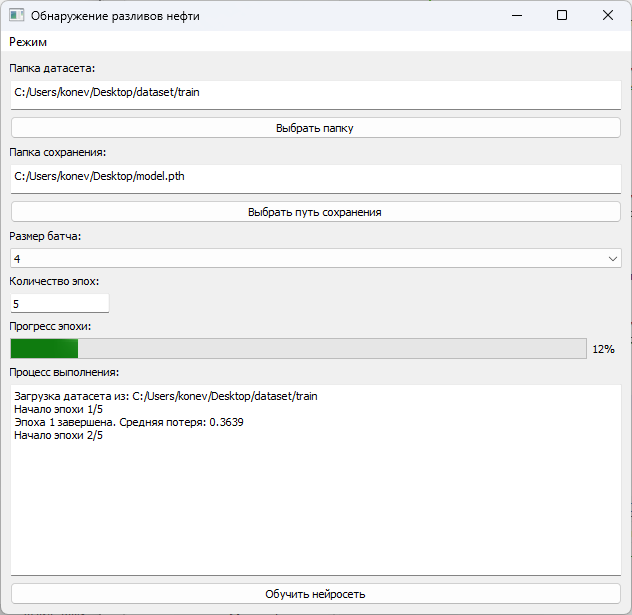
\includegraphics[width=0.7\linewidth]{images/обучение}
	\caption{Процесс обучения нейронной сети}
	\label{fig:training_process}
\end{figure}
\begin{figure}[H]
	\centering
	\includegraphics[width=0.7\linewidth]{"images/обучение результат"}
	\caption{Интерфейс программы после завершения обучения}
	\label{fig:training_result}
\end{figure}
\begin{figure}[H]
	\centering
	\includegraphics[width=0.5\linewidth]{"images/сохраненная модель"}
	\caption{Файл весов модели}
	\label{fig:saved_weights}
\end{figure}

На рисунке~\ref{fig:test_ui_default} изображено окно программы в режиме "<Тестирование">.
\begin{figure}[H]
	\centering
	\includegraphics[width=0.7\linewidth]{"images/тестирование интерфейс"}
	\caption{Окно режима "<Тестирование">}
	\label{fig:test_ui_default}
\end{figure}

На рисунке~\ref{fig:test_image_select} изображено диалоговое окно выбора тестового изображения.
\begin{figure}[H]
	\centering
	\includegraphics[width=0.7\linewidth]{"images/выбор анализируемого изображения"}
	\caption{Диалоговое окно выбора тестового изображения}
	\label{fig:test_image_select}
\end{figure}

На рисунке~\ref{fig:test_model_select} изображено диалоговое окно выбора тестируемых весов.
\begin{figure}[H]
	\centering
	\includegraphics[width=0.7\linewidth]{"images/выбор тестовой модели"}
	\caption{Диалоговое окно выбора тестируемой модели}
	\label{fig:test_model_select}
\end{figure}

На рисунке~\ref{fig:test_results_show} отображены результаты тестирования выбранных весов модели нейронной сети.
\begin{figure}[H]
	\centering
	\includegraphics[width=0.7\linewidth]{"images/результаты теста"}
	\caption{Результаты тестирования}
	\label{fig:test_results_show}
\end{figure}

\subsection{Сборка программной системы}

Программные компоненты представляют собой файлы исходных кодов программной системы.

Для сборки и компиляции программной системы использовалась библиотека Pyinstaller\cite{vasiliev-python}, позволяющая упаковать все необходимые файлы в один исполняемый файл формата .exe. Данный файл может быть запущен без предварительной установки.

Интерпретация исходных кодов на языке Python выполняется встроенным в исполняемый файл интерпретатором языка и не требует отдельной установки интерпретатора и библиотек на целевую систему.

Все программные компоненты собраны в один исполняемый файл, готовый к запуску в среде Windows.